\documentclass{article}
\usepackage[T1]{fontenc}
\usepackage[utf8]{inputenc}
\usepackage{spconf,amsmath,graphicx}
\usepackage{booktabs,tabularx,multirow,cite}
\usepackage[hidelinks]{hyperref}
\renewcommand{\thesection}{S\arabic{section}}
\renewcommand{\thesubsection}{\thesection.\arabic{subsection}}
\renewcommand{\thefigure}{S\arabic{figure}}
\renewcommand{\thetable}{S\arabic{table}}
\newcommand{\affmark}[1]{\textsuperscript{\fontsize{9}{10.8}\selectfont #1}}
\title{\fontsize{14}{16}\selectfont Supplementary Material for\\HY-MAST: Probing the Fragile Foundations of\\Music Understanding in Multimodal LLMs}
\name{\small yizou\affmark{1,2}, shangdawu\affmark{2}, liliangtang\affmark{2}, teddysun\affmark{2}, Qin Zhang\affmark{3}, ye long\affmark{4}, steveyves\affmark{2}, linus\affmark{2}}
\address{\small\begin{tabular}{@{}c@{}}
\affmark{1}School of Information and Communication Engineering, Communication University of China\\
\affmark{2}Hunyuan, Tencent\\
\affmark{3}State Key Laboratory of Media Convergence and Communication, Communication University of China\\
\affmark{4}School of Data Science and Intelligent Media, Communication University of China
\end{tabular}}
\hypersetup{pdftitle={HY-MAST: Supplementary Material},pdfauthor={yizou, shangdawu, liliangtang, teddysun, Qin Zhang, ye long, steveyves, linus}}

\begin{document}
\ninept
\raggedbottom
\makeatletter
\g@addto@macro\@maketitle{%
  \begin{minipage}{\textwidth}
    \centering
    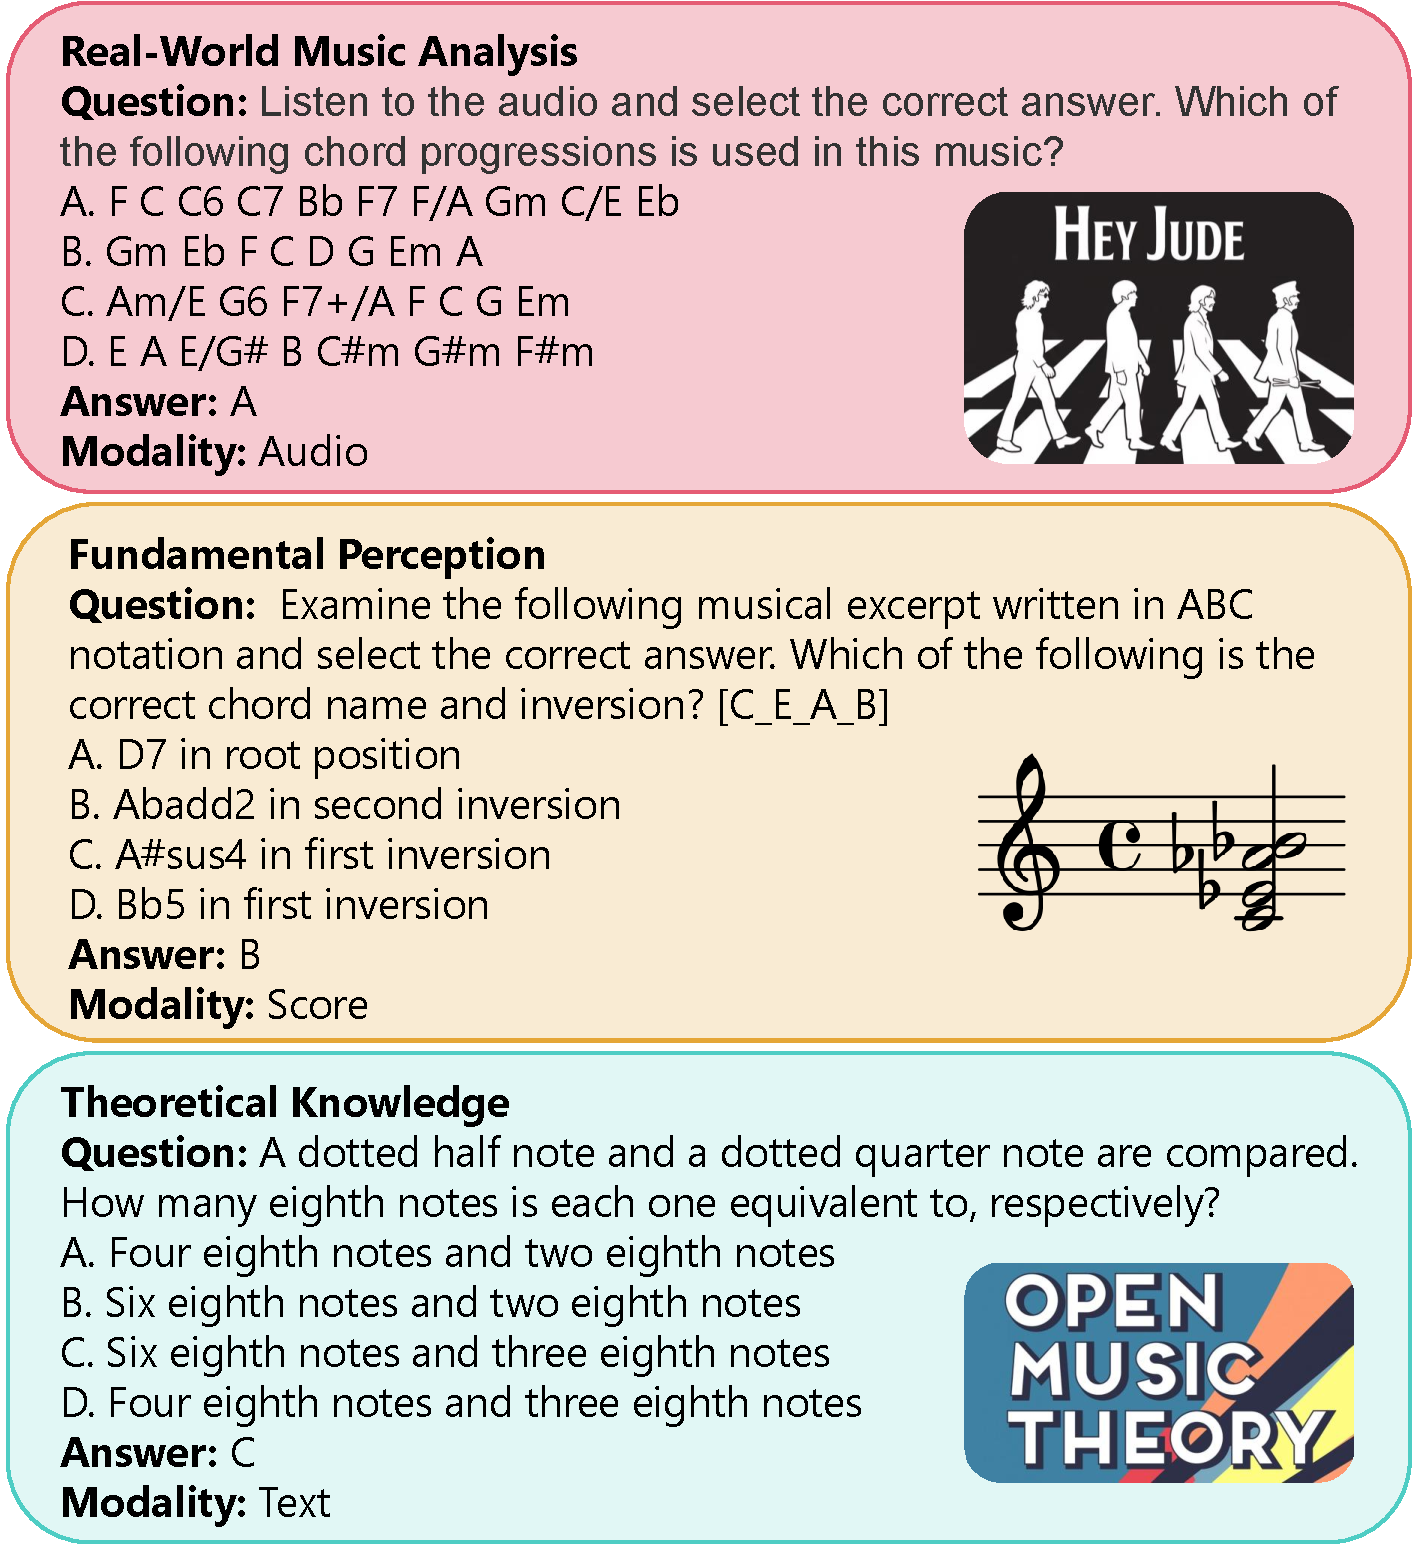
\includegraphics[width=0.61\textwidth]{demo.pdf}
    \def\@captype{figure}%
    \caption{Original example questions illustrating the three assessment components: real-world music analysis, fundamental perception, and theoretical knowledge.}
    \label{fig:examples}
  \end{minipage}
  \par\vspace{0.5em}
}
\makeatother
\maketitle

%\begin{abstract}This supplement preserves the extended motivation, benchmark construction, and evaluation condensed in the ICASSP 2027 main paper. References are numbered independently in the main paper and this supplement. Supplementary section, figure, and table numbers carry the prefix S.\end{abstract}

\section{Benchmark Construction Details}\label{sec:construction}
\subsection{Curated music corpus for Real-World music analysis}
This component assesses comprehensive understanding within real, complete, and complex works. Its tasks range from basic perception, such as tempo estimation, to integrated analysis, such as genre identification. 
\textbf{Popular music:} The entire Billboard \emph{Greatest of All Time Hot 100 Songs} chart is included. This historically aggregated chart provides the popular-music evaluation context. The original source is \url{https://www.billboard.com/charts/greatest-hot-100-singles/}. 
\textbf{Art music:} We manually select 100 representative MusicNet works~\cite{DBLP:conf/iclr/ThickstunHK17}, considering genre, period, and composer, to assess complex musical structure.
\textbf{World music:} We select 100 works from four regional collections associated with CompMusic~\cite{DBLP:conf/ismir/Serra11}: Arab-Andalusian music~\cite{DBLP:conf/dlfm/RepettoPCBS18}, the Jingju a cappella singing dataset~\cite{DBLP:conf/ismir/GongRS17}, Indian Carnatic and Hindustani music in Saraga~\cite{srinivasamurthy2021saraga}, and Turkish \c{s}ark{\i} vocal music~\cite{dzhambazov2014automatic}. 


\subsection{Fundamental perception generation}
The synthetic component tests core competencies under controlled conditions. Synthetic items can be generated in effectively unlimited numbers through two complementary methods.
\textbf{Rule-based generation.} Fragments target isolated musical elements: pitch in G3--G5, intervals within one octave, chords with at most four notes, rhythmic patterns, and scale-based tonality. A controlled, seed-driven pipeline generates each audio stimulus and corresponding ABC notation according to formal rules. Most pitch-related tasks present A4 before the target stimulus to mimic reference-based human testing conditions.
\textbf{Model-based generation.} Meter identification and melody transcription require coherent melodic phrases; isolated rule-based fragments lack the natural flow needed for these tasks. We train a lightweight Transformer decoder on the IrishMAN dataset~\cite{DBLP:conf/hcmir/WuLY023} to generate plausible short monophonic melodies in ABC notation. This component therefore contains both isolated-element and phrase-level items, not only single notes or chords.

\subsection{Theoretical knowledge construction}
This text-only examination contains 119 multiple-choice questions about formal music theory. Construction follows three stages:
\begin{enumerate}
\item A domain expert identifies the core concepts and extracts explanatory text from Open Music Theory~\cite{openmusictheory2021}.
\item DeepSeek-R1~\cite{DBLP:journals/corr/abs-2501-12948} uses the concept--text pairs to generate question stems, correct answers, and plausible distractors.
\item The expert reviews and refines the entire set for correctness, clarity, and appropriateness.
\end{enumerate}
Distractors are prompted to mirror the grammatical structure and stylistic register of the correct answer while containing a definite factual error. 
This design seeks to reduce guessing from superficial language patterns and make theoretical knowledge necessary for identifying the correct statement. 

\section{Evaluation Protocol}\label{sec:protocol}
\subsection{Prompt and scoring}
All evaluations use zero-shot, four-option multiple choice. The standardized instruction prepended to every model is:
\begin{quote}
\itshape Please answer the following multiple-choice question. You must choose the correct option letter (A, B, C, or D) and provide only the letter as your response. Question:
\end{quote}
Only the correct single-letter answer receives credit. Any non-conforming response is counted as incorrect. This strict protocol measures performance under a shared output constraint; transcription tasks are evaluated through candidate selection rather than unrestricted sequence generation.

\begin{table*}[t]
\centering
\caption{All original core-skill radar values (\%). A: audio; S: score; T: text. Am., St., Ex.: human amateurs, students, experts. GPT: GPT-4o-Audio; Kimi: Kimi-Audio-7B-Instruct; MiD: MiDashengLM-7B; MF: Music-Flamingo; Qwen: Qwen3.5-Omni-Plus; Gemini: Gemini-3.1-Pro.}
\label{tab:corevalues}
\setlength{\tabcolsep}{4pt}
\begin{tabularx}{\textwidth}{@{}Xrrrrrrrrr@{}}
\toprule
\textbf{Task} & \textbf{Am.} & \textbf{St.} & \textbf{Ex.} & \textbf{GPT} & \textbf{Kimi} & \textbf{MiD} & \textbf{MF} & \textbf{Qwen} & \textbf{Gemini}\\
\midrule
Pitch (A) & 66.7 & 71.4 & 100.0 & 30 & 22 & 24 & 28 & 96 & 99\\
Interval (A) & 58.3 & 71.4 & 90.5 & 29 & 22 & 22 & 20 & 33 & 51\\
Chord (A) & 50.0 & 57.1 & 71.4 & 21 & 19 & 15 & 38 & 47 & 44\\
Tonality (A) & 70.8 & 85.7 & 95.2 & 28 & 25 & 31 & 30 & 67 & 87\\
Rhythm (A) & 50.0 & 57.1 & 90.5 & 8 & 36 & 36 & 29 & 34 & 34\\
Meter (A) & 37.5 & 57.1 & 66.7 & 23 & 21 & 20 & 26 & 27 & 25\\
Melody (A) & 29.2 & 42.9 & 95.2 & 29 & 17 & 26 & 29 & 43 & 47\\
Interval (S) & 87.5 & 71.4 & 95.2 & 36 & 32 & 25 & 29 & 81 & 100\\
Chord (S) & 50.0 & 52.4 & 95.2 & 11 & 32 & 22 & 34 & 78 & 100\\
Tonality (S) & 58.3 & 47.6 & 90.5 & 24 & 32 & 50 & 39 & 93 & 100\\
Meter (S) & 25.0 & 47.6 & 90.5 & 1 & 20 & 22 & 23 & 31 & 64\\
Music theory (T) & 45.8 & 81.0 & 71.4 & 73 & 69 & 66 & 68 & 93 & 95\\
\bottomrule
\end{tabularx}
\end{table*}

\begin{table*}[t]
\centering
\caption{All original real-world radar values (\%). Model abbreviations follow Table~\ref{tab:corevalues}. A: audio; S: score.}
\label{tab:realvalues}
\begin{tabularx}{\textwidth}{@{}Xrrrrrr@{}}
\toprule
\textbf{Task} & \textbf{GPT} & \textbf{Kimi} & \textbf{MiD} & \textbf{MF} & \textbf{Qwen} & \textbf{Gemini}\\
\midrule
Genre (A) & 57 & 45 & 39 & 45 & 73 & 60\\
Instrument (A) & 45 & 27 & 23 & 49 & 80 & 58\\
Tempo (A) & 25 & 21 & 26 & 40 & 58 & 37\\
Meter (A) & 13 & 17 & 36 & 46 & 59 & 54\\
Tonality (A) & 25 & 17 & 18 & 45 & 44 & 50\\
Harmonic (A) & 30 & 22 & 24 & 59 & 65 & 76\\
Melody (A) & 21 & 20 & 26 & 24 & 40 & 29\\
Lyric (A) & 97 & 88 & 27 & 94 & 100 & 99\\
Work (A) & 67 & 56 & 39 & 75 & 86 & 84\\
Genre (S) & 26 & 19 & 30 & 25 & 26 & 52\\
Meter (S) & 12 & 18 & 43 & 56 & 66 & 68\\
Tonality (S) & 31 & 33 & 33 & 26 & 46 & 56\\
Work (S) & 39 & 18 & 28 & 18 & 38 & 52\\
\bottomrule
\end{tabularx}
\end{table*}

\subsection{Seed-controlled instantiation}
A random seed and configurable item counts instantiate an evaluation set. Researchers can change seeds or increase item counts to investigate performance anomalies or suspected overfitting. The default experiment uses the configuration described below. Seed control differs by component:
\begin{itemize}
\item \textbf{Real-world analysis:} the query work and distractors are sampled from the same sub-corpus. Distractors are valid labels within that context, reducing label-set exclusion shortcuts~\cite{DBLP:conf/ismir/ZangOBMN25}.
\item \textbf{Fundamental perception:} all musical materials and candidate options are generated algorithmically. The pipeline first creates four equally valid candidates, then randomly selects the target. The other candidates are incorrect only relative to the stimulus.
\item \textbf{Theoretical knowledge:} the 119 stems and their correct answers and distractors remain fixed. The seed changes the presentation order of the four options, preventing reliance on stable answer positions, not memorization of question content.
\end{itemize}

\section{Complete Radar Values}\label{sec:values}
Tables~\ref{tab:corevalues} and~\ref{tab:realvalues} preserve all values plotted in the two original radar figures. The main paper redraws those curves with compact axis labels and places dense numerical annotations here instead of superimposing them on intersecting curves. Axis order is unchanged. Human percentages retain the one-decimal values encoded in the original curves; model accuracies are integer percentages. Reported aggregate means and standard deviations remain unchanged in the main figures, including their original rounding.

\let\supplementbibliography\thebibliography
\renewcommand{\thebibliography}[1]{%
  \supplementbibliography{#1}%
  \setlength{\itemsep}{2pt}%
  \setlength{\parsep}{0pt}%
  \setlength{\parskip}{0pt}%
}
\bibliographystyle{IEEEbib}
\bibliography{ICASSP2027_refs}
\end{document}
